%
\documentclass{beamer}

% Customize slide appearance
%\mode<presentation>
{
  \usetheme{metropolis}
  \setbeamercovered{transparent}
}


\setbeamertemplate{navigation symbols}{} % don't use navigation tools on slides
\usepackage{graphicx}
\usepackage[absolute,overlay]{textpos}
%\usepackage{extrabeamercmds}    
\usepackage[loop,controls,buttonsize=0.24cm,buttonbg=0.8,autoplay]{animate}
\graphicspath{{./apollo17/}}

\usepackage[english]{babel}
\usepackage{times}

% You can add any graphics to every slide by following command:
% \logo{
\includegraphics{logo.eps}}

% Uncomment this, if you want the table of contents before each subsection.
% However, to edit slides in TeXWord avoiding this feature is good idea.
% \AtBeginSubsection[]
% {
%   \begin{frame}<beamer>
%     \frametitle{Outline}
%     \tableofcontents[currentsection,currentsubsection]
%   \end{frame}
% }

% If you wish to uncover everything in a step-wise fashion, uncomment
% the following command: 
%\beamerdefaultoverlayspecification{<+->}

\begin{document}

% Title Data. We keep it after \begin{document} 
% to enable editing text in BaKoMa TeX Word.

\title{Presentation Title}
\subtitle{Presentation Subtitle}

% Use the \inst command to identify several affiliations.
\author{F.~Author\inst{1} \and S.~Another\inst{2}}
\institute{
  \inst{1}%
  Department of Computer Science\\
  University of Somewhere
  \and
  \inst{2}%
  Department of Theoretical Philosophy\\
  University of Elsewhere}

\date[TUG 2005]{Annual TUG Conference, 2005}

\subject{Desktop Publishing} % Should be passed to PDF [YNI]

\begin{frame}
  \titlepage
\end{frame}

\begin{frame}
  \frametitle{Table of Contents}
  \tableofcontents
  Click TeX Refresh (F5) to update table of contents.
\end{frame}

\section{Videos}

%\ WORKS    
\begin{frame}
    \frametitle{Example 2}
    
    An example full frame video using the \textbf{basic syntax} is on this slide. This will play externally using default player.
    
    \vspace{20pt}
    
    \href{run:apollo17.avi}{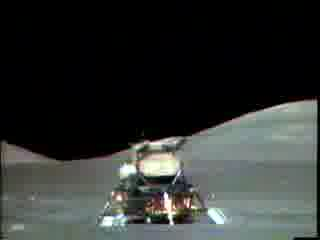
\includegraphics[height=0.7\textheight]{outputFrame_16.jpeg}}
\end{frame}

\begin{frame}
    \frametitle{Example 2: Test Graphics Path}
    
    An example of a single frame video using the graphics path.
    If this doesn't work, the next slide shouldn't work.
    
    \vspace{20pt}
    
    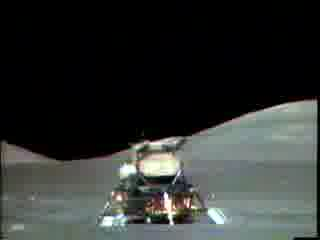
\includegraphics[height=0.7\textheight]{outputFrame_16.jpeg}
\end{frame}



\begin{frame}

\frametitle{Example using animate}
Here is an example using the animation package for playing within the pdf.
\begin{figure}
% here fps = 8, images are 1 through 42, show every image
\animategraphics[loop,width=.7\linewidth,every=1]{8}{outputFrame_}{1}{42}
\end{figure}
\end{frame}


% % DOES\ NOT\ WORK
% \begin{frame}
%     \frametitle{Example}
%     
%     An example full frame video using \textbf{commands from extrabeamercmds} is on the next slide. This does not work on Windows 10 or Ubuntu 15.10.
% 
% \fullFrameMovie[loop]{apollo17.avi}{apollo17.jpg}{\CopyrightText{Apollo 17, NASA}}
% \end{frame}
%     
% 
% 
% %\ DOES\ NOT\ WORK
% \begin{frame}
%     \frametitle{Example 3}
%     
%     An example full frame video using \textbf{commands from extrabeamercmds} is on the next slide. This does not work on Windows 10 or Ubuntu 15.10.
% 
% 
% % this assumes you have a .jpg named the same thing as your .avi
% \fullFrameMovieAvi[noloop]{apollo17}{\CopyrightText{Apollo 17, NASA}}
% \end{frame}
%     

\section{Introduction}

\subsection{General Features}

\begin{frame}
  \frametitle{Presentation Outline}
  \framesubtitle{Using sectioning commands}

  You can use \texttt{\textbackslash section}
  and \texttt{\textbackslash subsection} commands
  to define outline of your presentation.

  These commands must be appeared between frames.
  Insert they manually in text source window. 

  To take correct outline under \TeX-Word click F5 key.

\end{frame}

\begin{frame}
  \frametitle{Simple Overlays}
  \framesubtitle{Using pause command}

  The easiest way to create overlays is in using 
  the \texttt{\textbackslash pause} command.
  Like following ...

  \begin{itemize}
    \item This item is before \texttt{pause} (look source window)\pause
    \item If you don't see overlay read explanation below ...
  \end{itemize}

  Overlay expansion may be enabled/disabled 
  in dialog opened by `Insert/Document Properties' menu command.

  `\textit{Overlays Mode=\textbf{Handout}}' 
   -- disables overlay expansion.

  It is default setting of this template, 
  because this mode is convenient at
  first stage of developing slides.

  `\textit{Overlays Mode=\textbf{Beamer}}' 
   -- enables overlay expansion.

  It is useful at final editing 
  for handling overlays and for generating 
  final slides in form of PDF file.

\end{frame}

\subsection{Advanced Features}

\begin{frame}
  \frametitle{Advanced Overlays}
  \framesubtitle{Using more flexible overlay specifications}

  Beamer includes more ways for handling 
  overlays\dots
  \begin{itemize}
  \item using the \texttt{pause} command:
    \begin{itemize}
    \item
      First item.
      \pause
    \item    
      Second item.
    \end{itemize}
  \item
    using overlay specifications:
    \begin{itemize}
    \item<3->
      First item.
    \item<4->
      Second item.
    \end{itemize}
  \item
    using the general \texttt{uncover} command:
    \begin{itemize}
      \uncover<5->{\item
        First item.}
      \uncover<6->{\item
        Second item.}
    \end{itemize}
  \end{itemize}

  To learn more about Beamer package 
  read original documentation.

\end{frame}

\section{Main Talk}

\subsection{It is only beginning}

\begin{frame}
  \frametitle{Blank Frame}
  Body.
\end{frame}

\section*{Conclusion}

\begin{frame}
  \frametitle{Conclusion}

  Clicking right mouse button 
  (press+release without intermediate mouse moving) 
  displays context menu
  which have two commands specific for beamer package: 

  \begin{itemize}
  \item
     \alert{Delete the Frame} -- removes current frame.
  \item
     \alert{Duplicate the Frame} -- easiest frame populating.
  \end{itemize}

  The button 
  at left edge of text 
  tool bar lets you insert blank slide in your presentation.

\end{frame}


\end{document}




